\section{Megvalósítás}

Ebben a fejezetben részletesen bemutatásra kerül a rendszer  megvalósítása, a projekt kezdeti létrehozásától kezdve a mappa- és fájlstruktúra leírásán át a legfontosabb funkciók implementációjáig. A cél egy átláthatóan felépített alkalmazás létrehozása , amely mind a felhasználói, mind az adminisztratív felületen stabil és könnyen karbantartható működést biztosít.


\subsection{A projekt létrehozása és környezet beállítása}

A fejlesztés Microsoft Visual Studio 2022 környezetben valósult meg, a .NET 8.0 keretrendszerre építve. A projekt típusa \textit{ASP.NET Core MVC Web Application}, amely a model-view-controller (MVC) architektúra elveit követi, lehetővé téve az üzleti logika, a megjelenítés és az adatkezelés hatékony rendszerezését.

Az adatkezeléshez az Entity Framework Core komponenst használtam, a Code First megközelítés segítségével. Entity Framework Core, egy modern ORM technológia a .NET alkalmazások számára, amely lehetővé teszi az adatbázis-műveletek magas szintű megvalósítását. Ennek köszönhetően a modell osztályok a programkódban lettek definiálva, majd migrációk létrehozásával az adatbázis-struktúra automatikusan generálódott. Ez a módszer rugalmasságot biztosít a fejlesztés során, és egyszerűsíti az adatbázis módosítását.

Az alkalmazás egy SQL Server Express alapú relációs adatbázist használ, amely helyi környezetben gyors, megbízható és könnyen konfigurálható megoldást biztosít a fejlesztéshez. Az adatbázis kezelése teljesen az Entity Framework migrációs rendszerére épül.


\subsection{A megvalósítás mappastruktúrája és fő komponensei}

A projekt létrehozása a Visual Studio 2022 fejlesztőkörnyezet és a .NET 8 keretrendszer segítségével valósul meg. Az így generált mappastruktúra jól rendszerezett, illetve könnyen bővíthető, támogatja az átlátható fejlesztést és megkönnyíti az egyes komponensek logikai szétválasztását.

A \texttt{Controllers} mappa felelős azokért az osztályokért, amelyek a felhasználói interakciókat kezelik és az adatokat feldolgozzák a működési logika szerint. Ezek a vezérlők külön-külön foglalkoznak az egyes entitásokkal, például a menetrendekkel, jegyekkel vagy felhasználókkal, biztosítva az adatok és a nézetek közötti kapcsolatot.

A \texttt{Models} könyvtár tartalmazza azokat az osztályokat, amelyek az adatbázisban tárolt entitásokat képezik, például a \texttt{Ticket}, \texttt{Contact} vagy \texttt{Schedule} osztályokat. Ezek az osztályok felelősek az adatok szerkezetének és az entitások közötti kapcsolatok megvalósításáért. Tulajdonképpen az adatbázis tábláinak a mintája

A felhasználói felület komponensei, vagy másnéven nézetek a \texttt{Views} mappában találhatóak. A nézetek logikusan szerveződnek az egyes vezérlőkhöz tartozó almappákba, amelyek tartalmazzák az adott entitáshoz kapcsolódó Razor nézeteket, például \texttt{Index}, \texttt{Details}, \texttt{Edit}.

A \texttt{wwwroot} mappa biztosítja az alkalmazás statikus tartalmainak tárolását, mint például a képek, design-ért felelős komponensek (CSS), valamint JavaScript fájlok. Ezek a fájlok közvetlenül kiszolgálhatók a kliens számára, így támogatják a weboldal vizuális megjelenését és interaktív működését.

A \texttt{Data} mappa tartalmazza az \texttt{AppDbContext} osztályt, amely az adatmodell és az adatbázis összekapcsolásához szükséges.

Különálló mappaként jelenik meg a \texttt{Migrations} könyvtár is, amely az Entity Framework által generált migrációs fájlokat foglalja magában. Ezek az entitások naplózzák az adatmodellben történt változásokat, lehetővé téve az adatbázis fokozatos és szabályozott módosítását fejlesztés közben.

A fent bemutatott mappastruktúra jól átgondolt rendszert biztosít az alkalmazás különböző részeinek elválasztásához, elősegítve ezzel a tiszta kódszervezést, a hatékony fejlesztést és a későbbi karbantartást.

\subsection{Adatmodell és adatbázis felépítése}

Miután a projektet létrehoztuk, elsőként az alkalmazás alapját képező osztályokat, azaz a modelleket kellett létrehozni. Ezek az osztályok az adatbázisban tárolt adattáblákat írják le, és tartalmazzák a hozzájuk tartozó tulajdonságokat, valamint az egymással képzett relációkat. Az előzetesen elkészített adatbázis-terv alapján hoztam létre  a \texttt{AdminMessage}, \texttt{AdminRask}, \texttt{Attachment}, \texttt{Bus}, \texttt{Contact}, \texttt{RouteStop}, \texttt{Schedule}, \texttt{Stop}, \texttt{Ticket}, valamint \texttt{TransportRoute}. Itt fontos kritérium volt figyelni arra, hogy az entitások között pontosan és figyelmesen implementáljauk a relációkat. Itt gondolok az elsődleges kulcsok(Primary Key), illetve az idegen kulcsok(Foreign Key) helyes használatára.

A Contact osztályomat az ASP.NET Identity komponensének az IdentityUser ősosztályából származtattam, amely egy beépített megoldást kínál a felhasználók szerepkörének a zökkenőmentes implementálására, illetve használatára.

A modellek és az adatbázis közötti kapcsolatot az \texttt{AppDbContext} osztály biztosítja, amely az Entity Framework Core egyik központi komponense. Ez az osztály a \texttt{IdentityDbContext} ősosztályból származik, és célja az, hogy konfigurálja, kezelje és összekapcsolja a modelleket, sablonként szolgálva. Az \texttt{AppDbContext} osztályban találhatóak a \texttt{DbSet<T>} típusú tulajdonságok, amelyek egy-egy tábla leképezését valósítják meg, például: public DbSet<Stop> Stops { get; set; }, public DbSet<Schedule> Schedules { get; set; }.

Ezen felül az \texttt{AppDbContext} lehetőséget biztosít az entitások viselkedésének testreszabására az \texttt{OnModelCreating} metódusban, ahol külön definiálhatjuk a kulcsokat, kapcsolatokat, korlátozásokat, valamint egyéb konfigurációkat. Különösen hasznos az úgynevezett „vizesés törlés” (cascade delete) viselkedés figyelembe vétele, amely során egy entitás törlése vízesésszerüen magával vonhatja más kapcsolódó entitások törlését is. Az \texttt{OnModelCreating} metódus lehetőséget biztosít ennek felügyelésére, ezáltal elkerülve az adatvesztést okozó nem kívánt láncfolyamatokat.

\begin{figure}[H]
\centering
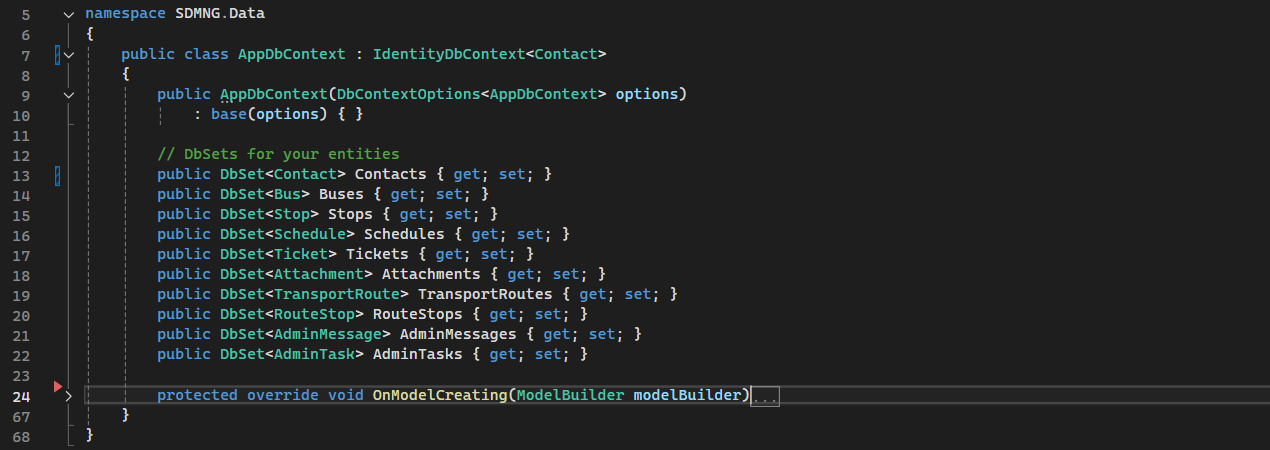
\includegraphics[width=1\textwidth]{Szakdolgozat/Mellekletek/AppDbContext.PNG}
\caption{A projektem AppDbContext osztálya látható az általam definiált modellekkel kiegészítve. }
\label{fig:appdbcontext}
\end{figure}

A \ref{fig:appdbcontext}. ábrán látható, a rendszeremben létrehozott osztályok segítségével létrehozott struktúra, amely a helyes adatbázis megvalósításában játszik kulcsszerepet. Az AppDbContext nevű osztályt az IdentityDbContext ősosztályból származtattam, majd egészítettem ki.
\vspace{\baselineskip}


Az AppDbContext osztály beállítása után szükség volt az adatbázis-fájl konfigurálására. A projekt \texttt{appsettings.json} fájlban megadtuk az adatbázis elérési útvonalát a \texttt{ConnectionStrings} szekcióban.

\begin{figure}[H]
\centering
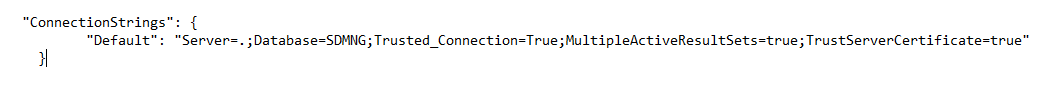
\includegraphics[width=1\textwidth]{Szakdolgozat/Mellekletek/Connectionstring.PNG}
\caption{Az adatbázis kapcsolódási kulcsa a lokális adatbázishoz.}
\label{fig:connectionstring}
\end{figure}

A \ref{fig:connectionstring}. ábrán a projektben használt \textit{connection string} látható, amely a lokális SQL Server adatbázishoz való kapcsolódást valósítja meg. Ez tartalmazza az SDMNG adatbázis elérési útvonalát, az adatbázis nevét, valamint a hitelesítési mód beállításait.
\vspace{\baselineskip}

A továbbiakban, mikor a konfigurációs fájlok helyesen vannak implementáva, meg a modell osztályaink is terv szerint lettek megvalósítva, kész voltam az első migráció hozzáadására. Az adatbázis létrehozását az Entity Framework migrációs rendszere segítségével oldottam meg. Az első migráció elkészítéséhez a terminálban a következő parancsot adtuk ki: 
\begin{lstlisting}
dotnet ef migrations add CreateDatabase
\end{lstlisting}
A parancs végrehajtása után a Migrations mappában létrejött a fentebb megadott névvel rendelkező migrációs fájl. Itt fontos mégegyszer ellenőrizni a generálodott adatbázis entitásait, illetve különös hangsúlyt kell fekteni a relációk ellenőrzésére. Amennyiben minden a terv szerint valósult meg, akkor végrehajtjuk  az adatbázis fizikai létrehozása vagy frissítésére használt parancsot parancsot: 
\begin{lstlisting}
dotnet ef database update
\end{lstlisting}

Ez a parancs a korábban generált migrációs fájlok alapján felépíti vagy kiegészíti az adatbázist a megadott kapcsolati karakterlánc (connection string) segítségével.

\subsubsection{Menetrendek (Schedules)}



\subsubsection{Jegyek (Tickets, MyTicket oldal)}



\subsubsection{Kapcsolatfelvétel (Contact Us)}



\subsubsection{Felhasználói fiókok és jogosultságkezelés}



\subsubsection{Buszok és mellékletek kezelése}



\subsection{Navigáció és UI integráció}



\subsection{Hibakezelés és validáció}


